\documentclass[12pt]{article}
\usepackage[a4paper, text={17cm,24cm}, top=3cm, left=1.5cm]{geometry}
\usepackage[utf8]{inputenc}
\usepackage{times}
\usepackage[czech]{babel}
\usepackage[unicode]{hyperref}
\usepackage{graphicx}
\usepackage{cprotect}
\usepackage{multirow}


\begin{document}

\begin{titlepage}
	\begin{center}

		
\includegraphics[height = 150pt]{img/FIT_barevne_CMYK_CZ.pdf} \\

		\begin{LARGE}
			\textsc{FAKULTA INFORMAČNÍCH TECHNOLOGIÍ} \\
			\textsc{VYSOKÉ UČENÍ TECHNICKÉ V BRNĚ}
		\end{LARGE}
		\\[5mm]
		
		\begin{LARGE}
			\textbf{Formální jazyky a překladače} 
		\end{LARGE}
        \\[20mm]
		\begin{Large}
				\textbf{Dokumentace projektu do IFJ a IAL} 
		\end{Large}
		\\[20mm]
		\begin{Large}
				\textbf{Tým 066, varianta II} 
		\end{Large}
		\\[20mm]
\begin{table}[h]
\centering
\begin{large}	
\catcode`\-=12
    \begin{tabular}{l l l l}
         Roman Ondráček & xondra58 & \% & vedoucí\\
         Pavel Raur & xraurp00 & \% &\\
         František Jeřábek & xjerab25 & \% &\\
         Radim Lipka & xlipka02 & \% & 
    \end{tabular}
\end{large}
\end{table}
\vfill
\begin{Large}
				\textbf{Seznam implementovaných rozšíření}
\end{Large}
\\[5mm]
\begin{Large}
			    \textsc{boolop, base, funexp, ifthen tabunary} 
\end{Large}
\end{center}
\end{titlepage}

\tableofcontents
\newpage
\section{Úvod}
Tento dokument byl vytvořen jako dokumentace společného projektu do předmětů Formální jazyky a pře\-kla\-da\-če a Algoritmy. Jsou zde popsány postupy implementace jednotlivých komponent překladače a problémy spojené s jejich implementací.
\section{Rozbor částí překladače}
Zadáním bylo vytvořit překladač jazyka \textbf{IFJ19}, který je podmnožinou jazyka Python 3, do cílového jazyka \textbf{IFJcode19}.
Jelikož se jedná o variantu projektu II, bylo nutné implementovat tabulku symbolů implementovat jako tabulku s rozptýlenými položkami.
\\
Implementovaný překladač se dělí na několik dílčích modulů:
\begin{itemize}
  \item Lexikální analyzátor
  \item Syntaktický analyzátor
  \item Sémantický analyzátor
  \item Generátor cílového kódu
\end{itemize}
Při samotném překladu se tedy dostane ke slovu jako první lexikální analyzátor, poté přijde na řadu syntaktický analyzátor se sémantickou analýzou a následně generátor cílového kódu. 
\subsection{Lexikální analýza}
Úkol lexikálního analyzátoru je načítat jednotlivé lexikální jednotky (lexémy) a převádět je na jednotlivé tokeny, které reprezentují daný lexém v dalších částech překladače. 

Část lexikální analýzy překledače je naimplementována v modulu \textbf{scanner.c} pomocí \textit{konečného stavového automatu}, který byl pro tuto část překladače navrhnut. Nerozpoznatelný vstupní token je označen \textsc{t\_unknown} a token reprezentující interní chybu překladače, například chybu alokace paměti \textsc{t\_error}.

Důležitou součástí lexikální analýzy překladače jazyka IFJ19 je také zásobníkový automat, který je použit pro práci s odsazením jednotlivých řádků vstupního souboru.
\begin{figure}[!htbp]
    \centering
    \scalebox{0.70}{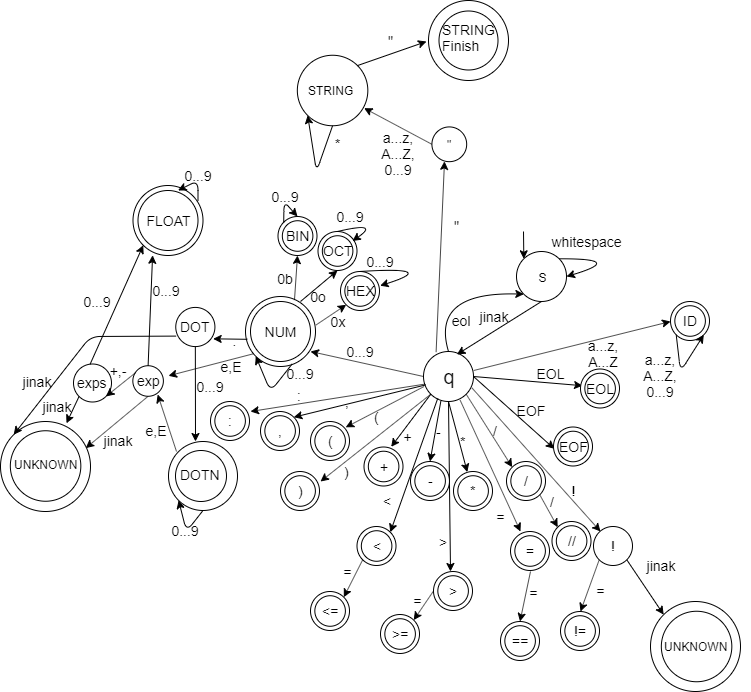
\includegraphics{img/Lexical_Analysis.png}}
    \caption{Automat lexikální analýzy}
    \label{obr:1}
\end{figure}
\clearpage
\subsection{Syntaktická analýza}
Implementace syntaktické analýzy se nachází v modulu \textbf{parser.c}. Jedná se o implementaci metodou shora dolů, konkrétněji metodou \textit{rekurzivního sestupu}, která je založena na LL--gramatice a LL--tabulce.

Vstupem syntaktické analýzy jsou jednotlivé tokeny z lexikální analýzy.

Jedním z úkolů syntaktické analýzy je naplnění tabulky symbolů.
\subsubsection{LL--Gramatika a LL--Tabulka}
\begin{enumerate}
    \item $<$code$>$ $\rightarrow$ $<$body$>$  $<$eols$>$  EOF
    \item $<$body$>$ $\rightarrow$ $<$definitions$>$ $<$statements$>$
    \item $<$definitions$>$ $\rightarrow$ $<$eols$>$ $<$definition$>$ $<$definitions$>$
    \item $<$definition$>$ $\rightarrow$ $\epsilon$
    \item $<$definition$>$ $\rightarrow$ DEF IDENTIFIER ($<$function\_params$>$) : $<$eols$>$ INDENT $<$statements$>$ DEDENT
    \item $<$definition$>$ $\rightarrow$ $<$function\_call$>$
    \item $<$function\_call$>$ $\rightarrow$ IDENTIFIER ($<$function\_params$>$)
    \item $<$function\_params$>$ $\rightarrow$ $\epsilon$
    \item $<$function\_params$>$ $\rightarrow$ $<$function\_param$>$ $<$function\_nparam$>$
    \item $<$function\_nparam$>$ $\rightarrow$ , $<$function\_param$>$ $<$function\_nparam$>$
    \item $<$function\_nparam$>$ $\rightarrow$ $\epsilon$
    \item $<$function\_param$>$ $\rightarrow$ IDENTIFIER
    \item $<$statements$>$ $\rightarrow$ $\epsilon$
    \item $<$statements$>$ $\rightarrow$ $<$statement$>$ EOL $<$eols$>$ $<$statements$>$
    \item $<$statement$>$ $\rightarrow$ $<$returnRule$>$
    \item $<$statement$>$ $\rightarrow$ $<$condition$>$
    \item $<$statement$>$ $\rightarrow$ $<$asignment$>$
    \item $<$statement$>$ $\rightarrow$ $<$whileRule$>$
    \item $<$statement$>$ $\rightarrow$ PASS
    \item $<$returnRule$>$ $\rightarrow$ RETURN $<$return\_expression$>$
    \item $<$return\_expression$>$ $\rightarrow$ $\epsilon$
    \item $<$return\_expression$>$ $\rightarrow$ ($<$return\_expression$>$)
    \item $<$return\_expression$>$ $\rightarrow$ $<$expression$>$
    \item $<$condition$>$ $\rightarrow$ IF $<$condition\_expression$>$: EOL $<$eols$>$ INDENT $<$statement$>$ DEDENT $<$else\_condition$>$
    \item $<$else\_condition$>$ $\rightarrow$ $\epsilon$
    \item $<$else\_condition$>$ $\rightarrow$ ELSE : EOL $<$eols$>$ INDENT $<$statement$>$ DEDENT
    \item $<$condition\_expression$>$ $\rightarrow$ ($<$condition\_expression$>$)
    \item $<$condition\_expression$>$ $\rightarrow$ $<$expression$>$
    \item $<$asignment$>$ $\rightarrow$ IDENTIFIER = $<$expression$>$
    \item $<$whileRule$>$ $\rightarrow$ WHILE $<$condition\_expression$>$ : EOL $<$eols$>$ INDENT $<$statement$>$ DEDENT
    \item $<$eols$>$ $\rightarrow$ $\epsilon$
    \item $<$eols$>$ $\rightarrow$ EOL $<$eols$>$
\end{enumerate}

\begin{table}[!htbp]
\catcode`\-=12
\centering
    \begin{tabular}{|c|c|c|c|c|c|c|c|c|c|c|c|c|c|c|c|c|c|}
    \hline
       & {\rotatebox[origin=c]{90}{DEF}} & {\rotatebox[origin=c]{90}{ID}} & (
       & ) & {\rotatebox[origin=c]{90}{INDENT}} & {\rotatebox[origin=c]{90}{DEDENT}} & {\rotatebox[origin=c]{90}{RETURN}} & {\rotatebox[origin=c]{90}{IF}} & {\rotatebox[origin=c]{90}{ELSE}} & : & {\rotatebox[origin=c]{90}{WHILE}} & {\rotatebox[origin=c]{90}{PASS}} & {\rotatebox[origin=c]{90}{EOF}} & {\rotatebox[origin=c]{90}{EOL}} & = & ,\\ 
    \hline
        $<$code$>$ & 1 & 1 &  &  &  &  &  &  &  &  &  &  &  & 1 &  &\\
    \hline
        $<$body$>$ & 2 & 2 &  &  &  &  &  &  &  &  &  &  &  & 2 &  &\\
    \hline
        $<$defs$>$ & 3 & 3 &  &  &  &  &  &  &  &  &  &  &  & 3 &  &\\
    \hline
        $<$def$>$ & 5 & 6 &  &  &  &  &  &  &  &  &  &  &  &  &  &\\
    \hline
        $<$f\_call$>$ &  & 7 &  &  &  &  &  &  &  &  &  &  &  &  & &\\
    \hline
       $<$f\_params$>$&  & 9 &  &  &  &  &  &  &  &  &  &  &  &  &  &\\
    \hline
        $<$f\_nparam$>$ &  & 10 &  &  &  &  &  &  &  &  &  &  &  &  &  & 10\\
    \hline
        $<$f\_param$>$ &  & 12 &  &  &  &  &  &  &  &  &  &  &  &  &  &\\
    \hline
        $<$stats$>$ &  &  &  &  &  &  &  &  &  &  &  &  &  &  &  &\\
    \hline
        $<$stat$>$ &  & 17 &  &  &  &  & 15 & 16 &  &  & 18 & 19 &  &  &  &\\
    \hline
        $<$retRule$>$ &  &  &  &  &  &  & 20 &  &  &  &  &  &  &  &  &\\
    \hline
        $<$ret\_exp$>$ &  &  & 22 &  &  &  &  &  &  &  &  &  &  &  &  &\\
    \hline
        $<$condition$>$ &  &  &  &  &  &  &  & 24 &  &  &  &  &  &  &  &\\
    \hline
        $<$else\_cond$>$ &  &  &  &  &  &  &  &  & 26 &  &  &  &  &  &  &\\
    \hline
        $<$cond\_exp$>$ &  &  & 27 &  &  &  &  &  &  &  &  &  &  &  &  &\\
    \hline
        $<$assignment$>$ &  & 29 &  &  &  &  &  &  &  &  &  &  &  &  &  &\\
    \hline
        $<$whileRule$>$ &  &  &  &  &  &  &  &  &  &  & 30 &  &  &  &  &\\
    \hline
        $<$eols$>$ & 31 & 31 & 31 & 31 & 31 & 31 & 31 & 31 & 31 & 31 & 31 & 31 & 31 & 32 & 31 & 31\\
    \hline
    \end{tabular}
    \caption{LL--Tabulka}
    \label{tab:1}
\end{table}
\subsubsection{Precedenční syntaktická analýza}
Precedenční syntaktická analýza je využita pro zpracování výrazů a je řízena přecedenční tabulkou. Stejně jako syntaktická analýza je precedenční analýza implementována v modulu \textbf{parser.c}.

Jelikož bylo implementováno i rozšíření \textsc{tabunary}, bylo potřeba se vypořádat s rozdílem mezi unárními operátory plus a mínus a jejich binární podobou, protože do této části syntaktické analýzy přicházejí jako od sebe nerozpoznatelné tokeny. 

V precedenční analýze je hojně využit zásobník. Každý příchozí token je porovnáván s aktuálním obsahem vrcholu zásobníku a podle predenční tabulky je prováděna náležitá operace. Ty jsou typicky dvě, buď je zpracovávaný token pouze uložen na zásobník nebo je uvolněn aktuální vrchol zásobníku. Ten je redukován podle jednoho z předem definovaných pravidel. Výraz se takto postupně zpracováná a postupně redukuje, dokud není dosažen konec zpracovávaného výrazu, který je symbolizován znakem \textbf{\$}. Stejný znak je na začátku precedenční analýzy vložen na vrchol zásobníku, takže posledním porovnáním u každého výrazu, který je bez chyby, je porovnání \textbf{\$} s \textbf{\$}. Po dokončení všech redukcí a po nalezení konce výrazu tedy vznikná výsledný strom.
\begin{table}[!htbp]
\catcode`\-=12
\centering
    \begin{tabular}{l l l}
         E $\rightarrow id$ & E $\rightarrow$ E $+$ E & E $\rightarrow$ E $<$ E \\
         E $\rightarrow $ (E) & E $\rightarrow$ E $-$ E & E $\rightarrow$ E $>$ E \\
         E $\rightarrow id$() & E $\rightarrow$ E $*$ E & E $\rightarrow$ E $<=$ E \\
         E $\rightarrow id$(E) & E $\rightarrow$ E $/$ E & E $\rightarrow$ E $>=$ E \\
         E $\rightarrow id$(E, ...) & E $\rightarrow$ E $//$ E & E $\rightarrow$ E $and$ E \\
         E $\rightarrow$ E $==$ E & E $\rightarrow$ E $!=$ E & E $\rightarrow$ E $or$ E \\
         E $\rightarrow not$ E & &  \\
    \end{tabular}
    \caption{Redukční pravidla}
    \label{tab:2}
\end{table}
\begin{table}[!htbp]
\catcode`\-=12
\centering
    \begin{tabular}{|c|c|c|c|c|c|c|c|c|c|c|c|c|c|c|c|c|c|c|}
    \hline
       & $*$ & $/$ & $//$ & $+$ & $-$ & $<$ & $>$ & $<=$ & $>=$ & $==$ & $and$ & $or$ & $not$ & $!=$ & $($ & $)$ & $id$ & $\$$\\ 
    \hline
        $*$ & $>$ & $>$ & $>$ & $>$ & $>$ & $>$ & $>$ & $>$ & $>$ & $>$ & $>$ & $>$ & $<$ & $>$ & $<$ & $>$ & $<$ & $>$\\
    \hline
        $/$ & $>$ & $>$ & $>$ & $>$ & $>$ & $>$ & $>$ & $>$ & $>$ & $>$ & $>$ & $>$ & $<$ & $>$ & $<$ & $>$ & $<$ & $>$\\
    \hline
        $//$ & $>$ & $>$ & $>$ & $>$ & $>$ & $>$ & $>$ & $>$ & $>$ & $>$ & $>$ & $>$ & $<$ & $>$ & $<$ & $>$ & $<$ & $>$\\
    \hline
        $+$ & $<$ & $<$ & $<$ & $>$ & $>$ & $>$ & $>$ & $>$ & $>$ & $>$ & $>$ & $>$ & $<$ & $>$ & $<$ & $>$ & $<$ & $>$\\
    \hline
        $-$ & $<$ & $<$ & $<$ & $>$ & $>$ & $>$ & $>$ & $>$ & $>$ & $>$ & $>$ & $>$ & $<$ & $>$ & $<$ & $>$ & $<$ & $>$\\
    \hline
        $<$ &  $<$ & $<$ & $<$ & $<$ & $<$ & $-$ & $-$ & $-$ & $-$ & $-$ & $>$ & $>$ & $<$ & $-$ & $<$ & $>$ & $<$ & $>$\\
    \hline
        $>$ & $<$ & $<$ & $<$ & $<$ & $<$ & $-$ & $-$ & $-$ & $-$ & $-$ & $>$ & $>$ & $<$ & $-$ & $<$ & $>$ & $<$ & $>$\\
    \hline
        $<=$ & $<$ & $<$ & $<$ & $<$ & $<$ & $-$ & $-$ & $-$ & $-$ & $-$ & $>$ & $>$ & $<$ & $-$ & $<$ & $>$ & $<$ & $>$\\
    \hline
        $>=$ & $<$ & $<$ & $<$ & $<$ & $<$ & $-$ & $-$ & $-$ & $-$ & $-$ & $>$ & $>$ & $<$ & $-$ & $<$ & $>$ & $<$ & $>$\\
    \hline
        $==$ & $<$ & $<$ & $<$ & $<$ & $<$ & $-$ & $-$ & $-$ & $-$ & $-$ & $>$ & $>$ & $<$ & $-$ & $<$ & $>$ & $<$ & $>$\\
    \hline
        $and$ & $<$ & $<$ & $<$ & $<$ & $<$ & $<$ & $<$ & $<$ & $<$ & $<$ & $>$ & $>$ & $<$ & $<$ & $<$ & $>$ & $<$ & $>$\\
    \hline
        $or$ & $<$ & $<$ & $<$ & $<$ & $<$ & $<$ & $<$ & $<$ & $<$ & $<$ & $<$ & $>$ & $<$ & $<$ & $<$ & $>$ & $<$ & $>$\\
    \hline
        $not$ & $>$ & $>$ & $>$ & $>$ & $>$ & $>$ & $>$ & $>$ & $>$ & $>$ & $>$ & $>$ & $<$ & $>$ & $<$ & $>$ & $<$ & $>$\\
    \hline
        $!=$ & $<$ & $<$ & $<$ & $<$ & $<$ & $-$ & $-$ & $-$ & $-$ & $-$ & $>$ & $>$ & $<$ & $-$ & $<$ & $>$ & $<$ & $>$\\
    \hline
        $($ & $<$ & $<$ & $<$ & $<$ & $<$ & $<$ & $<$ & $<$ & $<$ & $<$ & $<$ & $<$ & $<$ & $<$ & $<$ & $=$ & $<$ & $-$\\
    \hline
        $)$ & $>$ & $>$ & $>$ & $>$ & $>$ & $>$ & $>$ & $>$ & $>$ & $>$ & $>$ & $>$ & $>$ & $>$ & $-$ & $>$ & $-$ & $>$\\
    \hline
        $id$ & $>$ & $>$ & $>$ & $>$ & $>$ & $>$ & $>$ & $>$ & $>$ & $>$ & $>$ & $>$ & $>$ & $>$ & $=$ & $>$ & $-$ & $>$\\
    \hline
        $\$$ & $<$ & $<$ & $<$ & $<$ & $<$ & $<$ & $<$ & $<$ & $<$ & $<$ & $<$ & $<$ & $<$ & $<$ & $<$ & $-$ & $<$ & $-$\\
    \hline
    \end{tabular}
    \caption{Tabulka precedenční syntaktické analýzy}
    \label{tab:3}
\end{table}

\subsection{Sémantická analýza}
Sémantické kontroly jsou přidruženy k rekurzivnímu sestupu syntaktické analýzy.
Naimplementovány jsou v modulu \textbf{semantic\_analysis.c}. Největší část sémantických kontrol spočívá v kontrole datových typů výrazů, které vstupují do různých operací. V případě nejednotnosti těchto datových typů poté probíhá implicitní přetypování. Jelikož byla implementována podpora rozšíření \textsc{boolop}, kromě implicitního přetypování z typu \emph{int} na \emph{float}, je nutné podporovat i přetypování z typu \emph{bool} na \emph{int} a \emph{float}.

\subsection{Generátor cílového kódu}
Generátor cílového kódu byl implementován v modulu \textbf{inter\_code\_generator.c}. Úkolem tohoto modulu je vytvářet cílový kód, tedy v našem případě kod \textbf{IFJcode19}.
\subsection{Optimalizace}
\subsection{Tabulka symbolů a další datové struktury}
Tabulka symbolů je implementována jako tabulka s rozptýlenými položkami v modulu \textbf{symtable.c}. Tabulka symbolů uchovává informace o všech jednotkách vyskytujích se ve vstupním programu. 

Pro práci s různě dlouhými vstupními řetezci byl v modulu \textbf{dynamic\_string.c} implementován datový typ dynamický string. V lexikální analýze je také použit již dříve zmíněný zásobník v modulu \textbf{stack.c} pro práci s různýmy úrovněmi zanoření lexémů.


Precedenční analýza poté pracuje se zásobníkem z modulu \textbf{tree\_element\_stack.c}, na kterém pro\-bí\-há porovnávání vrcholu tohoto zásobníku s nově přicházejícími tokeny.

\section{Implementovaná rozšíření}
\subsection{BOOLOP}
Pro implementaci rozšíření BOOLOP byla přidána další pravidla do precedenční analýzy, konkrétně pravidla pro \textbf{not, or, and} a \textbf{==} a zároveň další sémantická pravidla pro kontrolu datových typů vstupujících do těchto operací.

\subsection{BASE}
Implementace rozšíření BASE spočívá v přidání a vypořádání se s dalším způsobem zadávání čí\-sel\-ných konstant. Do lexikální analýzy byly přidány stavy pro přijímání lexémů konstant zapsaných v binární, oktalové a hexadecimální soustavě, jejich převod na tokeny a předání dalším částem pře\-kla\-da\-če.

\subsection{FUNEXP}
Rozšíření FUNEXP požadovalo podporu volání funkce jako součást výrazu a také výrazy jako parametry funkce při jejím volání. Do precedenční analýzy pro to byla přidány pravidla, která toto umožňují.

\subsection{IFTHEN}
V rozšíření IFTHEN se měl podporovat ternární operátor, \textbf{elif}, a konstrukce \textbf{if} bez části \textbf{else}. Právě poslední zmíněné rozšíření je naším překladačem podporováno.

\subsection{TABUNARY}
V rozšíření TABUNARY se mělo rozlišovat mezi unárním a bi\-nár\-ním mínusem a plusem v precedenční analýze a podporou odsazování jak pomocí mezer, tak pomocí tabulátorů i prolínání těchto dvou způsobů odsazení. Část tohoto rozšíření, ve které se mělo rozlišovat právě mezi binárními a unárními operátory nebyla implementována. Pro část rozšíření, která se týká odsazování pomocí tabulátorů bylo třeba rozšířit zásobík u lexikální analýzy, aby bral v úvahu i tabulátory a ne jenom mezery.

\section{Týmová spolupráce}
Od začátku řešení projektu jsme se pravidelně scházeli nejdříve přibližně jedenkrát týdně a s blížícím se termínem odevzdání poté i vícekrát za týden. Pro rychlou komunikaci mezi sebou v reálném čase jsme si zvolili službu \textbf{Slack.com}, kde jsme ihned řešili všechny problémy, které nastaly.

Jako verzovací systém jsme použili \textbf{Git} hostovaný na stránce \textbf{GitHub}. 
\subsection{Rozdělení práce}
\begin{itemize}
  \item Roman Ondráček
  \item Pavel Raur
  \item František Jeřábek
  \item Radim Lipka
\end{itemize}
\section{Závěr}
Cílem projektu bylo pochopit a prakticky si vyzkoušet metody a techniky vysvětlované v předmětech IFJ a IAL a ze všeho nejvíc pochopit, z čeho se skládá překladač a jak fungují jeho jednotlivé části. 

Práce na projektu, ať už studium teorie, návrhy nebo samotná implementace nám přinesla řadu zkušeností, nových znalostí a rozšířila nám obzory na poli překladačů, jazyků a algoritmů.
\section{Použitá literatura, nástroje, programy}
\begin{itemize}
  \item Alexandr Meduna a Roman Lukáš, Formální jazyky a překladače, prezentace k přednáškám
  \item Jan M. Honzík, Ivana Burgetová, Bohuslav Křena, Algoritmy, prezentace k přednáškám
  \item Zbyněk Křivka a Radim Kocman, Demonstrační cvičení IFJ, Implementace překladače IFJ19 
  \item cppreference.com, \href{https://en.cppreference.com/}{https://en.cppreference.com/}
  \item GitHub, \href{https://github.com/}{https://github.com/}
  \item Slack, \href{https://slack.com/}{https://slack.com/}
\end{itemize}
\end{document}